\documentclass[border=10pt]{standalone}
\usepackage{pgfplots}
\pgfplotsset{compat=1.18}
\begin{document}
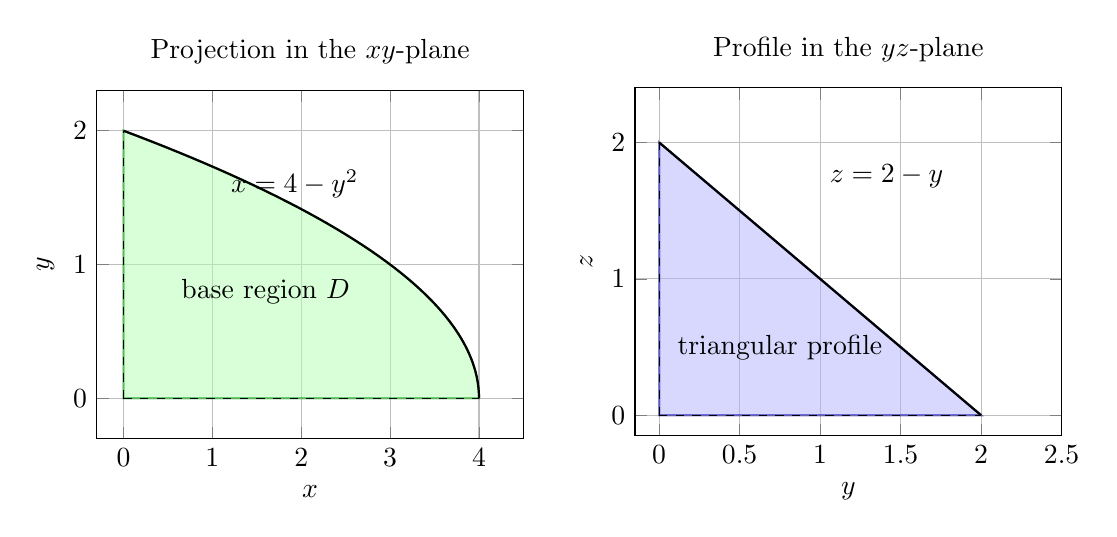
\begin{tikzpicture}
% Left: xy-plane projection
\begin{axis}[
    name=leftax,
    width=7cm, height=6cm,
    xlabel = {$x$}, ylabel = {$y$},
    xmin=-0.3, xmax=4.5, ymin=-0.3, ymax=2.3,
    title={Projection in the $xy$-plane},
    grid=major, domain=0:2, samples=50,
]
\addplot[green!60!black, fill=green!30, opacity=0.5, thick]
    ({4-x^2}, {x}) -- (0,0) -- cycle;
\addplot[black, thick, domain=0:2] ({4-x^2}, {x});
\addplot[black, dashed] coordinates {(0,0) (0,2)};
\addplot[black, dashed] coordinates {(0,0) (4,0)};
\node[anchor=west] at (axis cs:1.1,1.6) {$x=4-y^2$};
\node at (axis cs:1.6,0.8) {base region $D$};
\end{axis}
% Right: yz-plane profile
\begin{axis}[
    at={(leftax.outer east)}, anchor=outer west, xshift=0.6cm,
    width=7cm, height=6cm,
    xlabel = {$y$}, ylabel = {$z$},
    xmin=-0.15, xmax=2.5, ymin=-0.15, ymax=2.4,
    title={Profile in the $yz$-plane},
    grid=major, domain=0:2, samples=2,
]
\addplot[blue!60!black, fill=blue!30, opacity=0.5, thick]
    ({x}, {2-x}) -- (0,0) -- cycle;
\addplot[black, thick, domain=0:2] ({x}, {2-x});
\addplot[black, dashed] coordinates {(0,0) (0,2)};
\addplot[black, dashed] coordinates {(0,0) (2,0)};
\node[anchor=west] at (axis cs:1.0,1.75) {$z=2-y$};
\node at (axis cs:0.75,0.5) {triangular profile};
\end{axis}
\end{tikzpicture}
\end{document}